%-----------------------------------------------------------------------------------------------------------------
%% Section 1
\chapter{Question 1: Mass Actuator System}
\label{chap:q1}

As per \cite{assign}, it is required to find the natural frequency $\omega_n$ of the mass actuator system in Figure~\ref{fig:q1} below.

\begin{figure}[H]
	\centering
	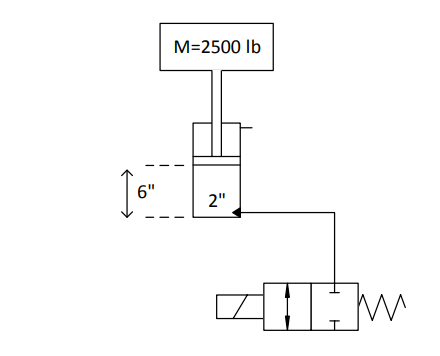
\includegraphics[scale=0.75]{q1}
	\caption{Circuit schematic.}
	\label{fig:q1}
\end{figure}

Constant parameters are listed in Table~\ref{tab:q1_param}. Furthermore, the following assumptions are made \cite{assign}.
\begin{itemize}
\item De-energized directional valve
\item Rigid cylinder walls
\item No air content
\end{itemize}

\begin{table}[H]
  \centering
  \caption{Given parameters.}
    \begin{tabular}{cccc}
    \textbf{Description} & \textbf{Symbol} & \textbf{Value } & \textbf{Unit} \\
    \midrule
    Mass  & $m$   & 2500  & lb \\
    Stroke & $l$   & 6     & in \\
    Diameter & $D$   & 2     & in \\
    Bulk modulus & $\beta$ & 260000 & psi \\
    \end{tabular}
  \label{tab:q1_param}
\end{table}

To find $\omega_n$ the system's dynamics must be derived. This is done with the hydraulics system equivalent model. Applying newtons second law to the free body diagram in Figure~\ref{fig:q1_fbd} will yield the final result in \ref{eq:q1_newt}.

\begin{figure}[H]
	\centering
	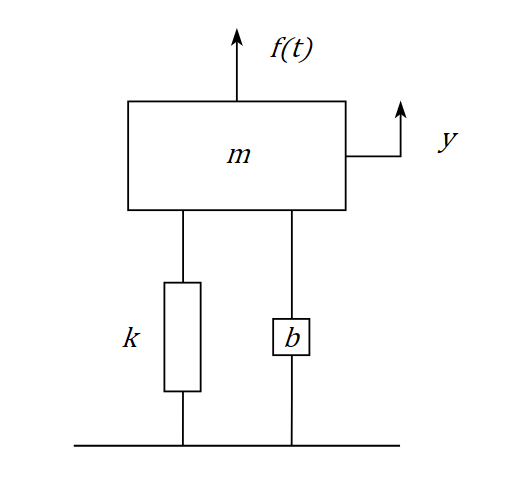
\includegraphics[scale=0.75]{q1_fbd}
	\caption{Free body diagram.}
	\label{fig:q1_fbd}
\end{figure}

\begin{equation}
	\label{eq:q1_newt}
	m \ddot{y} = f(t) - b\dot{y} - k y
\end{equation}

Taking the Laplace of \ref{eq:q1_newt} with zero initial conditions and rearranging to get in standard plant model form \ref{eq:q1_tfactual}.

\begin{equation*}
	ms^2 Y(s) + b s Y(s) + k Y(s) = F(s)
\end{equation*}

\begin{equation}
	\label{eq:q1_tfactual}
	P(s) = \frac{Y(s)}{F(s)} = \frac{\frac{1}{m}}{s^2 + \frac{b}{m}s + \frac{k}{m}}
\end{equation}

The natural frequency can be extrapolated from the ideal second order transfer function $P(s)$ \ref{eq:q1_tfideal}.
\begin{equation}
	\label{eq:q1_tfideal}
	P(s)= \frac{\omega_n^2}{s^2+2\zeta\omega_n s + \omega_n^2}
\end{equation}

Comparing like coefficients yields a final expression for $\omega_n$ \ref{eq:q1_wn}.
\begin{equation}
	\label{eq:q1_wn}	
	\omega_n = \sqrt{\frac{k}{m}}	
\end{equation}

Therefore need fluid equivalent of k.
\begin{equation}
	\label{eq:q1_beta}
	\beta = - \frac{\Delta p V_0}{\Delta V}	
\end{equation}

Realizing that $V_0 = AL$ and $\Delta V = Ax$, solving for $\Delta p$ yields the following

\begin{equation}
	\label{eq:q1_f}
	\Delta p = \frac{F}{A}= \beta \ \frac{y}{l} \Rightarrow F = \frac{A\beta}{l}y 	
\end{equation}

Knowing that $F = ky$, comparing the result of \ref{eq:q1_f} yields the final relation for the equivalent stiffness $k$

\begin{equation}
	\label{eq:q1_k}
	 k = \frac{A\beta}{l} 	
\end{equation}
 

%-----------------------------------------------------------------------------------------------------------------
%% Section 2
\chapter{Accumulator}
\label{chap:q2}


%-----------------------------------------------------------------------------------------------------------------
%% Section 3
\chapter{Cascade Design}
\label{chap:q3}
